% =============================================================================
% Section 16: Test Plan and Validation
% =============================================================================

\section{Test Plan and Validation}
\label{sec:test_plan}
\sectionauthors{BS, CM, JB, MN, JH, SC}

% -----------------------------------------------------------------------------
\subsection{Test Objectives and Scope}
% -----------------------------------------------------------------------------

The primary objective of this test plan is to systematically verify that the STAR Robot meets all functional and non-functional requirements defined in Section~\ref{sec:scope}. Testing serves two distinct purposes: verification (confirming the system is built correctly according to technical specifications) and validation (confirming the correct system is built to satisfy project requirements).

The scope of testing encompasses:

\begin{itemize}
    \item \textbf{Unit Verification:} Individual firmware drivers, mechanical components, and circuit modules tested in isolation.
    \item \textbf{Subsystem Integration:} Interaction between the ESP32-S3 firmware, Raspberry Pi 5 compute platform, electrical power systems, and mechanical chassis.
    \item \textbf{System Validation:} Full-stack ROS 2 navigation, SLAM Toolbox performance, and autonomous behavior under realistic indoor conditions.
\end{itemize}

The following items are explicitly out of scope: third-party ROS 2 libraries (assumed stable and treated as black-box components), manufacturing defects of off-the-shelf PCBs (assumed tested by vendor), and outdoor operation testing.

% -----------------------------------------------------------------------------
\subsection{Test Methodology: The V-Model Approach}
% -----------------------------------------------------------------------------

To ensure a structured validation process, this project utilizes the Systems Engineering V-Model, a framework that links each phase of the design lifecycle to a corresponding testing phase. The V-Model derives its name from its characteristic shape when visualized: the left arm represents progressive decomposition during design (from high-level requirements down to detailed component specifications), while the right arm represents progressive integration during testing (from unit tests up to acceptance testing).

The fundamental principle behind the V-Model is \textit{traceability}: every design decision should be verifiable through a corresponding test. This approach prevents the common pitfall of discovering defects late in development, where they are expensive to fix. Instead, the V-Model ensures that:

\begin{enumerate}
    \item Component Design is verified by Unit Testing: for example, verifying that the DRV8243-Q1 motor driver responds correctly to PWM signals from the ESP32-S3.
    \item Subsystem Design is verified by Integration Testing: for example, confirming that the ESP32-S3 correctly commands the motor drivers and receives encoder feedback via the SPI interface to the Raspberry Pi 5.
    \item System Requirements are validated by System Testing: for example, demonstrating that the robot can autonomously navigate a 50m path while avoiding obstacles (FR-001, FR-002).
    \item User Requirements are validated by Acceptance Testing: demonstrating the complete system to Dr. Porter and the review panel under real-world conditions.
\end{enumerate}

Figure~\ref{fig:v_model} illustrates this relationship. The horizontal dashed lines represent traceability links between design phases and their corresponding tests.

% TikZ Diagram for V-Model
\begin{figure}[H]
    \centering
    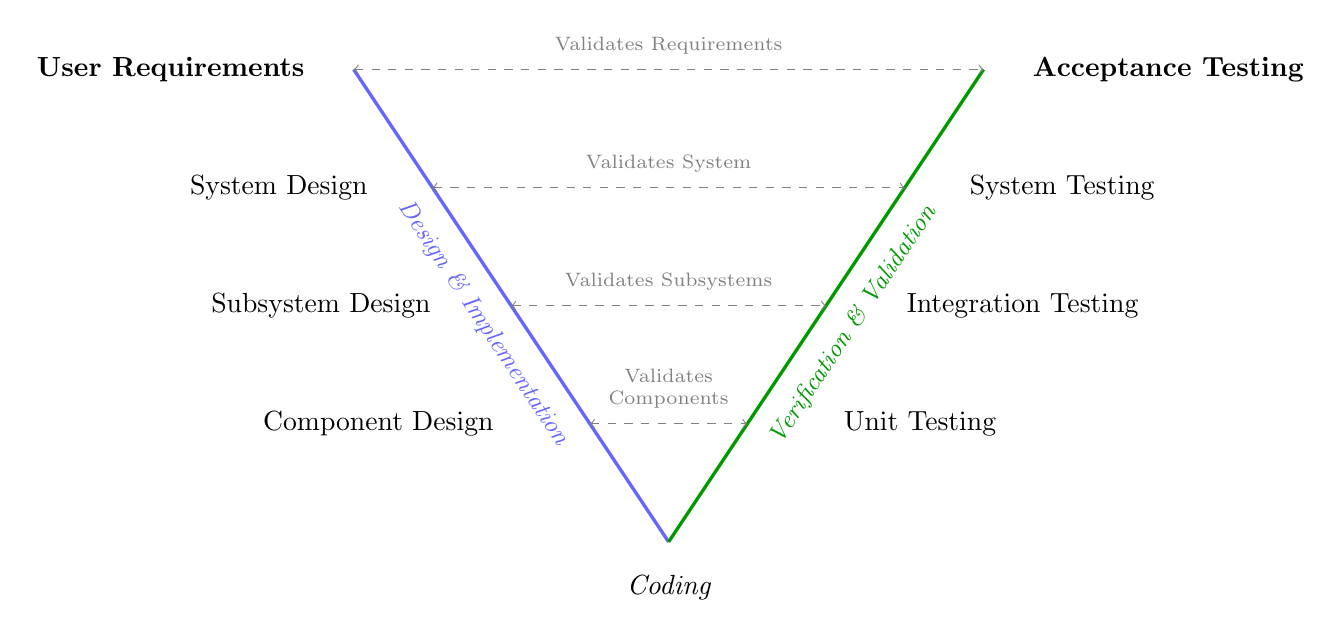
\begin{tikzpicture}[scale=1.0]
        % V-lines (as simple lines)
        \draw[very thick, blue!60] (0,6) -- (4,0);
        \draw[very thick, green!60!black] (4,0) -- (8,6);

        % Sloped labels for the V-lines, shifted to prevent overlap
        \path (0,6) -- (4,0) node [midway, sloped, font=\small, blue!60, yshift=-12pt] {\textit{Design \& Implementation}};
        \path (4,0) -- (8,6) node [midway, sloped, font=\small, green!60!black, yshift=-12pt] {\textit{Verification \& Validation}};

        % Left side (Design)
        \node[anchor=east, font=\normalsize\bfseries] at (-0.5, 6) {User Requirements};
        \node[anchor=east, font=\normalsize] at (0.3, 4.5) {System Design};
        \node[anchor=east, font=\normalsize] at (1.1, 3) {Subsystem Design};
        \node[anchor=east, font=\normalsize] at (1.9, 1.5) {Component Design};
        \node[anchor=north, font=\normalsize\itshape] at (4, -0.3) {Coding};

        % Right side (Testing)
        \node[anchor=west, font=\normalsize\bfseries] at (8.5, 6) {Acceptance Testing};
        \node[anchor=west, font=\normalsize] at (7.7, 4.5) {System Testing};
        \node[anchor=west, font=\normalsize] at (6.9, 3) {Integration Testing};
        \node[anchor=west, font=\normalsize] at (6.1, 1.5) {Unit Testing};

        % Traceability lines with corrected coordinates
        \draw[dashed, gray, <->] (0,6) -- (8,6);
        \node[font=\scriptsize, gray, above=2pt] at (4, 6) {Validates Requirements};

        \draw[dashed, gray, <->] (1,4.5) -- (7,4.5);
        \node[font=\scriptsize, gray, above=2pt] at (4, 4.5) {Validates System};

        \draw[dashed, gray, <->] (2,3) -- (6,3);
        \node[font=\scriptsize, gray, above=2pt] at (4, 3) {Validates Subsystems};

        \draw[dashed, gray, <->] (3,1.5) -- (5,1.5);
        \node[font=\scriptsize, gray, above=2pt, align=center] at (4, 1.5) {Validates\\Components};
    \end{tikzpicture}
    \caption{The V-Model approach applied to the STAR Robot validation strategy. The left arm represents design decomposition from user requirements to component specifications. The right arm represents verification and validation, progressing from unit tests to acceptance testing. Horizontal dashed lines indicate traceability between design phases and their corresponding tests.}
    \label{fig:v_model}
\end{figure}

% -----------------------------------------------------------------------------
\subsection{Test Strategy: The Testing Pyramid}
% -----------------------------------------------------------------------------

The test strategy follows the Testing Pyramid principle, which recommends a high volume of fast, automated unit tests at the base, fewer integration tests in the middle, and a small number of comprehensive system and acceptance tests at the top. This structure optimizes for rapid feedback: most defects are caught early by unit tests (which are fast and cheap to run), while integration and system tests catch issues that only emerge when components interact. Integration testing employs two complementary approaches: Hardware-in-Loop (HIL) testing runs software against physical hardware, while Software-in-Loop (SIL) testing uses simulation environments like Gazebo.

Figure~\ref{fig:test_pyramid} illustrates the pyramid structure. The width of each level represents the relative quantity of tests, while the height represents increasing integration complexity.

% TikZ Diagram for Testing Pyramid
\begin{figure}[H]
    \centering
    \begin{tikzpicture}[scale=1.0]
        % --- Pyramid Shape ---
        % Define main vertices
        \coordinate (V_BL) at (0,0);      % Vertex Bottom-Left
        \coordinate (V_BR) at (8,0);      % Vertex Bottom-Right
        \coordinate (V_TOP) at (4, 7.5);  % Vertex Top

        % Define y-levels for layers
        \def\yLvlOne{2}
        \def\yLvlTwo{4}
        \def\yLvlThree{6}

        % Calculate intersection points on the pyramid sides for filling
        \coordinate (P1L) at ($(V_BL)!\yLvlOne/7.5!(V_TOP)$);
        \coordinate (P1R) at ($(V_BR)!\yLvlOne/7.5!(V_TOP)$);
        \coordinate (P2L) at ($(V_BL)!\yLvlTwo/7.5!(V_TOP)$);
        \coordinate (P2R) at ($(V_BR)!\yLvlTwo/7.5!(V_TOP)$);
        \coordinate (P3L) at ($(V_BL)!\yLvlThree/7.5!(V_TOP)$);
        \coordinate (P3R) at ($(V_BR)!\yLvlThree/7.5!(V_TOP)$);

        % Fill layers with color (from bottom to top, lightest to darkest)
        \fill[blue!20] (V_BL) -- (V_BR) -- (V_TOP) -- cycle;
        \fill[blue!35] (P1L) -- (P1R) -- (V_TOP) -- cycle;
        \fill[blue!50] (P2L) -- (P2R) -- (V_TOP) -- cycle;
        \fill[blue!65] (P3L) -- (P3R) -- (V_TOP) -- cycle;

        % Draw outlines (main pyramid and dividers)
        \draw[thick] (V_BL) -- (V_BR) -- (V_TOP) -- cycle;
        \draw[thick] (P1L) -- (P1R);
        \draw[thick] (P2L) -- (P2R);
        \draw[thick] (P3L) -- (P3R);

        % --- Labels ---
        % Labels inside pyramid
        \node[font=\normalsize\bfseries] at (4, 1) {Unit Testing};
        \node[font=\normalsize\bfseries] at (4, 3) {Component Testing};
        \node[font=\normalsize\bfseries] at (4, 5) {Integration};
        \node[font=\small\bfseries] at (4, 6.7) {UAT};

        % Left side annotation (moved further left)
        \node[font=\small, align=right, anchor=east] at (-1.5, 3.5) {Increasing\\Integration\\Complexity};
        \draw[->, very thick] (-0.3, 0.5) -- (-0.3, 6.5);

        % Right side annotations
        \node[font=\small, align=left, anchor=west] (label1) at (9,1) {Many tests, fast,\\automated (Unity)};
        \node[font=\small, align=left, anchor=west] (label2) at (9,3) {Hardware drivers,\\sensor validation};
        \node[font=\small, align=left, anchor=west] (label3) at (9,5) {HIL/SIL testing,\\ROS 2 nodes};
        \node[font=\small, align=left, anchor=west] (label4) at (9,6.7) {Full robot,\\autonomous nav};

        % Arrows for right side annotations using projections
        \draw[<-, thick] ($(V_BR)!(label1.west)!(V_TOP)$) -- (label1.west);
        \draw[<-, thick] ($(V_BR)!(label2.west)!(V_TOP)$) -- (label2.west);
        \draw[<-, thick] ($(V_BR)!(label3.west)!(V_TOP)$) -- (label3.west);
        \draw[<-, thick] ($(V_BR)!(label4.west)!(V_TOP)$) -- (label4.west);
        
        % Bottom annotation
        \node[font=\small] at (4, -0.6) {Test Quantity $\rightarrow$};
    \end{tikzpicture}
    \caption{The Testing Pyramid showing the distribution of test types. Unit tests form the broad base with many fast, automated tests. Each successive level has fewer tests but validates increasingly complex integration. UAT = User Acceptance Testing.}
    \label{fig:test_pyramid}
\end{figure}

Table~\ref{tab:test_strategy} summarizes the five test levels employed in this project, from foundational unit tests to final acceptance testing.

\begin{table}[H]
    \centering
    \caption{Test Strategy Levels and Their Scope}
    \label{tab:test_strategy}
    \begin{tabular}{@{}clp{7cm}@{}}
        \toprule
        \textbf{Level} & \textbf{Test Type} & \textbf{Scope and Purpose} \\
        \midrule
        5 & Acceptance Testing & Validation against project requirements in real-world conditions (Final Demonstration, May 8, 2026) \\
        4 & System Testing & Complete integrated robot system operating autonomously in the test arena \\
        3 & Integration Testing & Interactions between subsystems using Hardware-in-Loop (HIL) and Software-in-Loop (SIL) methods \\
        2 & Component Testing & Individual hardware components and firmware drivers on the development bench \\
        1 & Unit Testing & Individual functions and modules tested in isolation using Unity Test Framework \\
        \bottomrule
    \end{tabular}
\end{table}

% -----------------------------------------------------------------------------
\subsection{Requirements Traceability}
% -----------------------------------------------------------------------------

Every test case is explicitly linked to one or more requirements from Tables~\ref{tab:functional_reqs} and~\ref{tab:nonfunctional_reqs} to ensure complete coverage. This traceability serves two purposes: it guarantees that all requirements are tested, and it allows impact analysis when requirements change.

The coverage objectives are:
\begin{itemize}
    \item 100\% of Critical and High priority requirements covered by at least one passed test case.
    \item $\geq$80\% code coverage for ESP32-S3 firmware modules (measured via Unity test framework).
    \item 100\% of hardware interfaces exercised during integration testing.
    \item All functional requirements (FR-001 through FR-009) validated by system-level tests.
\end{itemize}

% -----------------------------------------------------------------------------
\subsection{Test Items}
% -----------------------------------------------------------------------------

This section identifies all components subject to testing, organized by subsystem.

\subsubsection{Embedded Firmware Components}

Table~\ref{tab:firmware_items} lists the STAR firmware modules under test. Each module implements a specific abstraction layer (core services, bus communication, or sensor drivers) within the layered architecture described in Section~\ref{sec:embedded_impl}.

\begin{table}[H]
    \centering
    \caption{Embedded Firmware Test Items}
    \label{tab:firmware_items}
    \begin{tabular}{@{}llp{5.5cm}@{}}
        \toprule
        \textbf{ID} & \textbf{Component} & \textbf{Description} \\
        \midrule
        ESP-CORE-001 & star\_core & Abstract interfaces and system initialization \\
        ESP-ERR-001 & star\_error\_handler & Error handling with exponential backoff \\
        ESP-PIN-001 & star\_pin\_validator & GPIO conflict detection and validation \\
        ESP-BUS-001 & star\_bus & Unified I2C/SPI/UART bus abstraction \\
        ESP-DRV-003 & star\_sensor\_hcsr04 & Ultrasonic distance sensor driver (7 sensors) \\
        ESP-DRV-004 & star\_sensor\_bno055\_bmp280 & 10-DOF IMU + barometric pressure sensor \\
        ESP-DRV-005 & star\_bms\_bq78350 & Battery Management System SMBus driver \\
        \bottomrule
    \end{tabular}
\end{table}

\subsubsection{Electrical Subsystems}

Table~\ref{tab:electrical_items} identifies the electrical components requiring verification. Priority reflects the impact of failure on system safety and functionality.

\begin{table}[H]
    \centering
    \caption{Electrical Subsystem Test Items}
    \label{tab:electrical_items}
    \begin{tabular}{@{}lllc@{}}
        \toprule
        \textbf{ID} & \textbf{Component} & \textbf{Specification} & \textbf{Priority} \\
        \midrule
        ELE-PWR-001 & Power Distribution Board & 11.1V input, 3.3/5/6V regulated outputs & \cellcrit \\
        ELE-CHG-001 & BQ25798 Buck-Boost Charger & USB-C PD input, 3S LiPo charging & \cellcrit \\
        ELE-BMS-001 & BQ78350 Fuel Gauge & SMBus, state-of-charge monitoring & \cellcrit \\
        ELE-AFE-001 & BQ76920 AFE & Cell balancing, protection thresholds & \cellcrit \\
        ELE-MTR-001 & DRV8243-Q1 Motor Drivers ($\times$4) & 12V nominal, 8A peak per channel & \cellcrit \\
        ELE-IMU-002 & BNO055 + BMP280 Module & I2C, 9-axis fusion + pressure & \cellmed \\
        ELE-USS-001 & HC-SR04 Ultrasonic Sensors ($\times$7) & GPIO trigger/echo, 2--400cm range & \cellmed \\
        ELE-CAM-001 & IMX219-83 Stereo Camera & CSI-2 interface, V4L2 driver & \cellhigh \\
        \bottomrule
    \end{tabular}
\end{table}

\subsubsection{Mechanical Assemblies}

Table~\ref{tab:mechanical_items} lists the mechanical assemblies requiring structural and functional verification.

\begin{table}[H]
    \centering
    \caption{Mechanical Assembly Test Items}
    \label{tab:mechanical_items}
    \begin{tabular}{@{}lllc@{}}
        \toprule
        \textbf{ID} & \textbf{Component} & \textbf{Material/Type} & \textbf{Priority} \\
        \midrule
        MEC-CHS-001 & Robot Chassis & Aluminum frame, PETG panels & \cellcrit \\
        MEC-WHL-001 & Wheel Assemblies ($\times$4) & Rubber tires, custom bevel gears & \cellcrit \\
        MEC-ENC-001 & Wheel Encoders ($\times$4) & Optical quadrature, 360 CPR & \cellhigh \\
        MEC-MNT-001 & LiDAR Mount (SICK TiM561) & Machined aluminum & \cellhigh \\
        MEC-MNT-002 & Camera Mount (IMX219-83) & 3D printed PETG, adjustable angle & \cellmed \\
        MEC-MNT-003 & Electronics Enclosure & 3D printed PETG & \cellmed \\
        \bottomrule
    \end{tabular}
\end{table}

% -----------------------------------------------------------------------------
\subsection{Phase 1: Hardware and Electrical Verification}
% -----------------------------------------------------------------------------

Before any software deployment, the physical platform undergoes rigorous continuity testing and stress testing. This phase identifies manufacturing defects, assembly errors, and design issues that would otherwise cause confusing failures during software integration. All signal measurements utilize the RIGOL DHO804 digital oscilloscope, leveraging its 12-bit vertical resolution (4096 quantization levels) to detect low-amplitude noise and transients that 8-bit instruments would miss.

Table~\ref{tab:phase1_summary} summarizes the Phase 1 hardware verification tests. Complete test procedures and pass criteria are provided in Appendix~\ref{app:phase1_tests}.

\begin{table}[H]
    \centering
    \caption{Phase 1: Hardware Verification Test Summary}
    \label{tab:phase1_summary}
    \begin{tabular}{@{}llcl@{}}
        \toprule
        \textbf{Category} & \textbf{Test Range} & \textbf{Count} & \textbf{Key Verification Items} \\
        \midrule
        PCB Assembly & TC-PCB-001--006 & 6 & Power rails, signal traces, solder quality \\
        Power System & TC-PWR-001--007 & 7 & Rail accuracy ($\pm$3--10\%), protection circuits \\
        Communication & TC-COM-001--006 & 6 & I2C/SPI/UART integrity, bus enumeration \\
        Motor Control & TC-MTR-001--007 & 7 & Driver function, PWM, encoder feedback \\
        Mechanical & TC-MEC-001--008 & 8 & Structural load, alignment, thermal \\
        \midrule
        \textbf{Total} & & \textbf{34} & \\
        \bottomrule
    \end{tabular}
\end{table}

% -----------------------------------------------------------------------------
\subsection{Phase 2: Embedded Firmware Integration}
% -----------------------------------------------------------------------------

With hardware verified, Phase 2 tests the Hardware Abstraction Layer (HAL) and low-level drivers on the ESP32-S3. These tests execute on real hardware (Hardware-in-Loop testing) to verify that firmware correctly interfaces with the physical sensors and actuators. Table~\ref{tab:phase2_summary} summarizes the firmware integration tests; complete specifications are in Appendix~\ref{app:phase2_tests}.

\begin{table}[H]
    \centering
    \caption{Phase 2: Firmware Integration Test Summary}
    \label{tab:phase2_summary}
    \begin{tabular}{@{}llcl@{}}
        \toprule
        \textbf{Category} & \textbf{Test Range} & \textbf{Count} & \textbf{Key Verification Items} \\
        \midrule
        IMU Validation & TC-FW-001--002 & 2 & Gravity vector, gyroscope bias \\
        Odometry & TC-FW-003--004 & 2 & Distance accuracy ($<$2\%), PID tuning \\
        Timing/Safety & TC-FW-005--008 & 4 & Control loop (100Hz), watchdog, error handling \\
        Sensors & TC-FW-009 & 1 & Temperature-compensated ultrasonic \\
        \midrule
        \textbf{Total} & & \textbf{9} & \\
        \bottomrule
    \end{tabular}
\end{table}

% -----------------------------------------------------------------------------
\subsection{Phase 3: System Integration and ROS 2 Validation}
% -----------------------------------------------------------------------------

Phase 3 validates the complete robot stack, including the ROS 2 Humble middleware, SLAM Toolbox algorithms, Nav2 navigation planning, and the web-based user interface. These tests execute in the field test environment (described in Section~\ref{subsec:test_env}) using the fully assembled robot. Table~\ref{tab:phase3_summary} summarizes the system integration tests; complete specifications are in Appendix~\ref{app:phase3_tests}.

\begin{table}[H]
    \centering
    \caption{Phase 3: System Integration Test Summary}
    \label{tab:phase3_summary}
    \begin{tabular}{@{}llcl@{}}
        \toprule
        \textbf{Category} & \textbf{Test Range} & \textbf{Count} & \textbf{Key Verification Items} \\
        \midrule
        System Boot & TC-SYS-001--003 & 3 & Boot time, node health, latency \\
        SLAM/Navigation & TC-SYS-004--008 & 5 & Map quality, LiDAR, obstacle avoidance \\
        User Interface & TC-SYS-009--012 & 4 & Network, web UI, teleoperation \\
        Safety/Endurance & TC-SYS-013--015 & 3 & E-stop, battery life, CPU load \\
        \midrule
        \textbf{Total} & & \textbf{15} & \\
        \bottomrule
    \end{tabular}
\end{table}

% -----------------------------------------------------------------------------
\subsection{Test Environment and Tools}
\label{subsec:test_env}
% -----------------------------------------------------------------------------

Reproducible testing requires strictly controlled and documented environments. This section specifies the hardware, software, and physical spaces used for testing.

\subsubsection{Physical Test Environment}

\begin{table}[H]
    \centering
    \caption{Physical Test Environment Specifications}
    \label{tab:physical_env}
    \begin{tabular}{@{}p{3cm}p{9cm}@{}}
        \toprule
        \textbf{Environment} & \textbf{Configuration} \\
        \midrule
        \textbf{Development Bench} & Dedicated workstation with bench power supply, oscilloscope, and logic analyzer. Used for all Phase 1 and Phase 2 testing. Located in university fabrication lab. \\
        \midrule
        \textbf{Simulation (SIL)} & Gazebo Sim running on Ubuntu 22.04 with ROS 2 Humble. Used for algorithm validation before hardware deployment. Custom Buildroot image tested in QEMU. \\
        \midrule
        \textbf{Field Arena (HIL)} & 4m $\times$ 4m enclosed arena in university lab with variable lighting conditions (200--800 lux). Floor surfaces: tile (primary), concrete (secondary). Obstacles: static wooden blocks (various sizes) and wheeled carts for dynamic testing. \\
        \midrule
        \textbf{Extended Testing} & TEEX Disaster City complex available for realistic post-disaster scenario testing if schedule permits. \\
        \bottomrule
    \end{tabular}
\end{table}

\subsubsection{Test Equipment}

\begin{table}[H]
    \centering
    \caption{Laboratory Test Equipment}
    \label{tab:test_equipment}
    \begin{tabular}{@{}llp{5cm}@{}}
        \toprule
        \textbf{Equipment} & \textbf{Model} & \textbf{Purpose and Specification} \\
        \midrule
        Digital Oscilloscope & RIGOL DHO804 & Signal integrity, timing, and power analysis. 4 channels, 70MHz bandwidth, 12-bit vertical resolution (4096 levels). \\
        Logic Analyzer & HiLetgo USB & Bus protocol analysis (I2C, SPI, UART, SMBus). 8 channels, 24MHz sampling. \\
        Digital Multimeter & OWON XDM1041 & Precision voltage/current/resistance measurement. True RMS, 22000 count. \\
        Bench Power Supply & ATRIX MPS-6010H-1C ($\times$2) & Controlled power for HIL testing. 60V, 10A per unit. \\
        FTDI Adapter & FT232RL & Serial communication debug. 3.3V logic levels. \\
        \bottomrule
    \end{tabular}
\end{table}

\subsubsection{Software Test Environment}

\begin{table}[H]
    \centering
    \caption{Software and Tools Configuration}
    \label{tab:software_env}
    \begin{tabular}{@{}llp{5.5cm}@{}}
        \toprule
        \textbf{Tool} & \textbf{Version} & \textbf{Purpose} \\
        \midrule
        ESP-IDF & 5.x & ESP32-S3 SDK and toolchain \\
        PlatformIO & Latest & Build system and test runner for embedded \\
        Unity Test Framework & 2.5.x & Unit testing framework for C firmware \\
        Python & 3.10+ & Test automation scripts and data analysis \\
        ROS 2 & Humble Hawksbill & Robot middleware on custom Buildroot image \\
        Gazebo & Sim (Ignition) & Physics simulation for SIL testing \\
        Git/GitHub & Latest & Version control and issue tracking \\
        RViz2 & Humble & Real-time visualization of sensor data and maps \\
        \bottomrule
    \end{tabular}
\end{table}

% -----------------------------------------------------------------------------
\subsection{Defect Management}
% -----------------------------------------------------------------------------

When a test case fails, the defect enters a defined lifecycle to ensure systematic resolution and prevent regression.

\subsubsection{Severity Classifications}

Defect severity determines prioritization and blocking behavior:

\begin{itemize}
    \item \textbf{Critical (Blocker):} Safety hazard, system cannot boot, or data corruption. Testing of dependent components is blocked until resolved. Examples: motor runaway condition, power supply overvoltage, firmware crash on startup.
    \item \textbf{Major:} Key functionality fails (e.g., SLAM produces unusable maps), but workarounds exist or other subsystems can still be tested.
    \item \textbf{Minor:} Cosmetic issues, edge-case performance degradation, or documentation errors. Does not block other testing.
\end{itemize}

\subsubsection{Defect Lifecycle}

All defects follow this resolution process:

\begin{enumerate}
    \item \textbf{Log:} Defect recorded in GitHub Issues with severity label, reproduction steps, and expected vs. actual behavior.
    \item \textbf{Triage:} Team lead assigns priority and owner within 24 hours (Critical) or 72 hours (Major/Minor).
    \item \textbf{Isolate:} Developer reproduces the defect, preferably in the SIL environment for faster iteration.
    \item \textbf{Fix:} Code is patched and committed to a feature branch with a reference to the issue number.
    \item \textbf{Regression Test:} The original failing test \textit{and} all related tests are re-executed to ensure the fix does not introduce new faults.
    \item \textbf{Close:} Issue is marked closed only after the regression test passes and code is merged to main branch.
\end{enumerate}

% -----------------------------------------------------------------------------
\subsection{Entry and Exit Criteria}
% -----------------------------------------------------------------------------

Clear criteria govern transitions between test phases and final acceptance.

\subsubsection{Entry Criteria}

Each phase has prerequisites that must be satisfied before testing begins:

\begin{itemize}
    \item \textbf{Unit Testing:} Source code committed, compiles without errors or warnings, code review completed and approved.
    \item \textbf{Integration Testing:} All relevant unit tests pass (100\%), hardware available and powered, interface specifications documented.
    \item \textbf{System Testing:} All integration tests pass, robot fully assembled, power system verified safe by BS (Electrical Lead).
    \item \textbf{Acceptance Testing:} All system tests pass, user documentation complete, demonstration environment prepared.
\end{itemize}

\subsubsection{Exit Criteria}

Table~\ref{tab:exit_criteria} specifies the quantitative thresholds required to exit each phase.

\begin{table}[H]
    \centering
    \caption{Exit Criteria by Test Phase}
    \label{tab:exit_criteria}
    \begin{tabular}{@{}lllll@{}}
        \toprule
        \textbf{Phase} & \textbf{Execution} & \textbf{Pass Rate} & \textbf{Critical Defects} & \textbf{Coverage} \\
        \midrule
        Unit Testing & 100\% & $\geq 95\%$ & 0 open & $\geq 80\%$ code \\
        Integration Testing & 100\% & $\geq 90\%$ & 0 open & 100\% interfaces \\
        System Testing & 100\% & $\geq 85\%$ & 0 open & 100\% requirements \\
        Acceptance Testing & 100\% & 100\% & 0 open & Sponsor sign-off \\
        \bottomrule
    \end{tabular}
\end{table}

% -----------------------------------------------------------------------------
\subsection{Risk Assessment}
% -----------------------------------------------------------------------------

Table~\ref{tab:test_risks} identifies risks that could impact the testing schedule or outcomes, along with mitigation strategies. These risks complement the project-level risks documented in Section~\ref{sec:risks}.

\begin{table}[H]
    \centering
    \caption{Test Risk Register}
    \label{tab:test_risks}
    \begin{tabular}{@{}lp{3cm}ccp{4cm}@{}}
        \toprule
        \textbf{ID} & \textbf{Risk Description} & \textbf{Prob.} & \textbf{Impact} & \textbf{Mitigation Strategy} \\
        \midrule
        TR-001 & Hardware damage during testing & Med & High & Maintain spare components; enforce current-limited power-up procedures \\
        TR-002 & Firmware deadline overrun & Med & High & Begin integration testing early; parallelize with hardware verification \\
        TR-003 & Real-time performance insufficient & Med & High & Profile early; optimize critical paths; reduce logging in production \\
        TR-004 & GPIO overvoltage damage & Low & Critical & Implement strict pre-power voltage verification; use protective diodes \\
        TR-005 & Power system fault & Low & Critical & Fused connections; BMS monitoring; thermal shutoff via NTC thermistors \\
        TR-006 & SLAM accuracy below requirements & Med & High & Calibrate LiDAR carefully; tune SLAM Toolbox parameters; improve odometry \\
        TR-007 & Test environment unavailable & Low & Med & Schedule lab time in advance; maintain Gazebo simulation as backup \\
        \bottomrule
    \end{tabular}
\end{table}

% -----------------------------------------------------------------------------
\subsection{Quality Assurance Practices}
% -----------------------------------------------------------------------------

Quality is assured through multiple complementary mechanisms applied throughout the development and test cycle:

\begin{itemize}
    \item \textbf{Code Reviews:} All firmware and ROS 2 node changes require peer review and approval before merge to main branch.
    \item \textbf{Automated Regression:} CI/CD pipeline executes unit tests on every commit; integration tests run nightly on available hardware.
    \item \textbf{Design Reviews:} Formal review at each phase gate (PDR, Design Review, Final Demonstration) with documented decisions and action items.
    \item \textbf{Traceability:} Bidirectional links between requirements (FR/NFR), design documents, code, and test cases.
    \item \textbf{Documentation Review:} Technical documentation peer-reviewed for accuracy and completeness before milestone submissions.
\end{itemize}

% -----------------------------------------------------------------------------
\subsection{Tools and Development Environment}
% -----------------------------------------------------------------------------

\begin{table}[H]
    \centering
    \caption{Development Tools}
    \label{tab:dev_tools}
    \begin{tabular}{@{}lll@{}}
        \toprule
        \textbf{Category} & \textbf{Tool} & \textbf{Purpose} \\
        \midrule
        Version Control & Git/GitHub & Source code management, issue tracking \\
        IDE & CLion/VS Code & Development environment \\
        Testing & PlatformIO + Unity & Automated unit testing for ESP32-S3 \\
        Documentation & \LaTeX, Doxygen & Technical documentation, API references \\
        Project Management & Projectum & Custom task tracking aligned with WBS \\
        Visualization & RViz2 & Real-time sensor data and map visualization \\
        \bottomrule
    \end{tabular}
\end{table}

% -----------------------------------------------------------------------------
\subsection{Deployment and Acceptance Plan}
% -----------------------------------------------------------------------------

Final deployment follows a structured sequence aligned with project milestones (Table~\ref{tab:milestones}):

\begin{enumerate}
    \item \textbf{Final Assembly (M5):} Complete system integration with production firmware and calibrated sensors by March 31, 2026.
    \item \textbf{Software Integration (M6):} Functional ROS 2 software with navigation and mapping capabilities by April 15, 2026.
    \item \textbf{System Testing (M7):} Execute all system test cases in the university lab environment. Document results and resolve all Critical defects by May 1, 2026.
    \item \textbf{Documentation Delivery:} Provide user manual, assembly instructions, and software installation guide.
    \item \textbf{Final Demonstration (M8):} Present fully functional prototype to Dr. Porter and review panel on May 8, 2026. Execute acceptance test cases demonstrating autonomous mapping in real-world conditions.
    \item \textbf{Formal Handover:} Obtain signed acceptance; release all source code and hardware designs under MIT License on GitHub.
\end{enumerate}
